\documentclass[10pt,handout]{beamer}

\usetheme{Warsaw}

\usepackage{amsmath}
%\usepackage[style=apa]{biblatex}
\usepackage{multimedia}

\author{George G Vega\thanks{\url{mailto:gvegayon@caltech.edu}}}
\institute{Superintendencia de Pensiones}
\title{An\'alisis de Redes}
\date{27 de junio, 2014}

\begin{document}

\frame{\maketitle}

\begin{frame}
\frametitle{Contenidos}
\tableofcontents
\end{frame}


\section{Resiliencia}

\begin{frame}
\frametitle{Resiliencia de un grafo}

\begin{quote}
Un grafo $G$ (de una cierta clase) posee la propiedad $P$ [...] Qu\'e tan 
\emph{fuertemente} poseida se encuentra dicha propiedad? [...] Definimos
{\bf resiliencia} del grafo $G$ con respecto a $P$ como la medida que indica
que tanto debe cambiar $G$ para destruir $P$.
\end{quote} 

\begin{quote}
[...] ({\bf Resiliencia}) Sea $P$ una propiedad 
monot\'onicamente creciente. La resiliencia global de $G$ con respecto a $P$ es
el n\'umero m\'inimo $r$ tal que al eliminar $r$ arcos/vertices de $G$ resulta
en la p\'erdida de la propiedad $P$
\end{quote}
{\footnotesize Fuente: Adaptado de \cite{sudakov2008local}}
\end{frame}

\begin{frame}
\begin{figure}
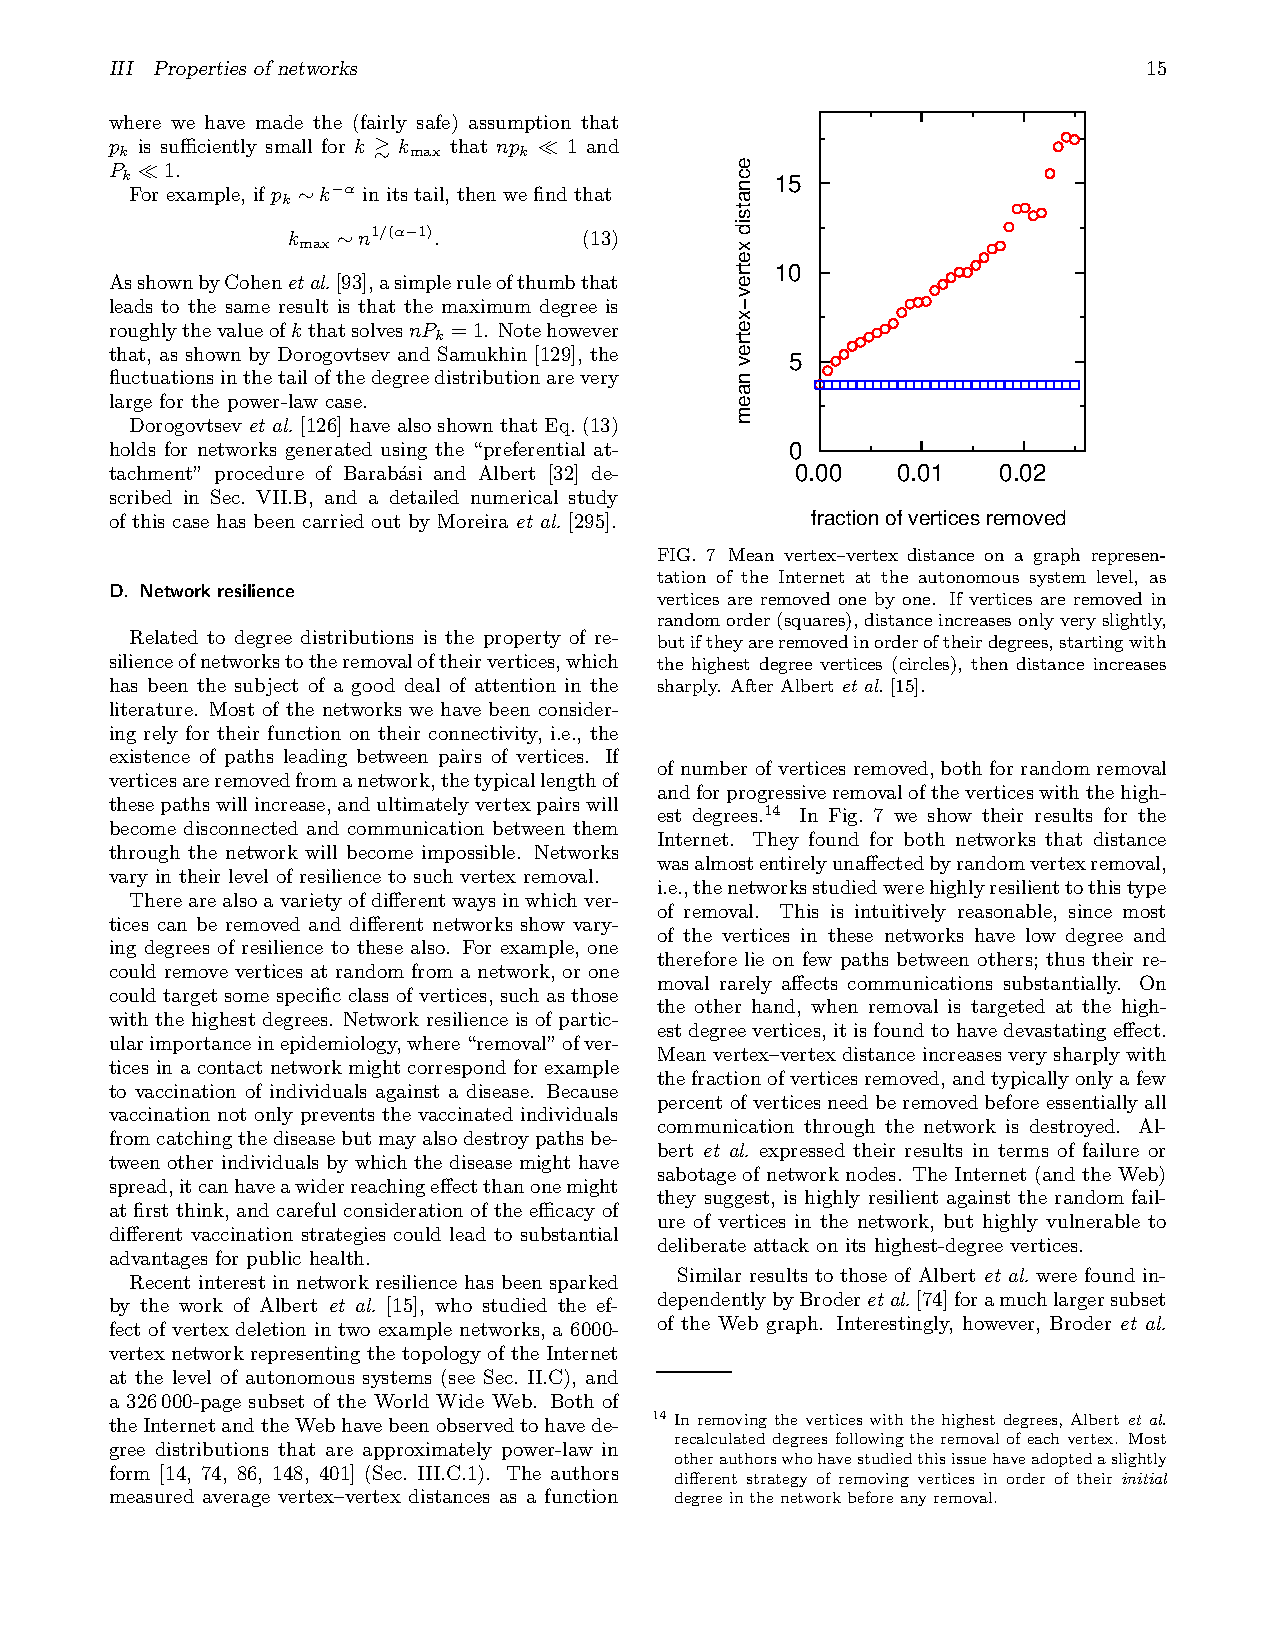
\includegraphics[trim=11cm 16cm 1.5cm 1.5cm, clip=true, width=.6\linewidth]{newman_network_resilense.pdf}
\end{figure}
{\footnotesize Fuente: Extraido del curso \emph{Social Network Analysis}, Lada
Adamic, University of Michigan \cite{lada2014}}
\end{frame}

\section{Homofilia (assortative mixing)}

\begin{frame}
\frametitle{Homofilia (assortative mixing)}
\begin{figure}
\centering
% trim=l b r t
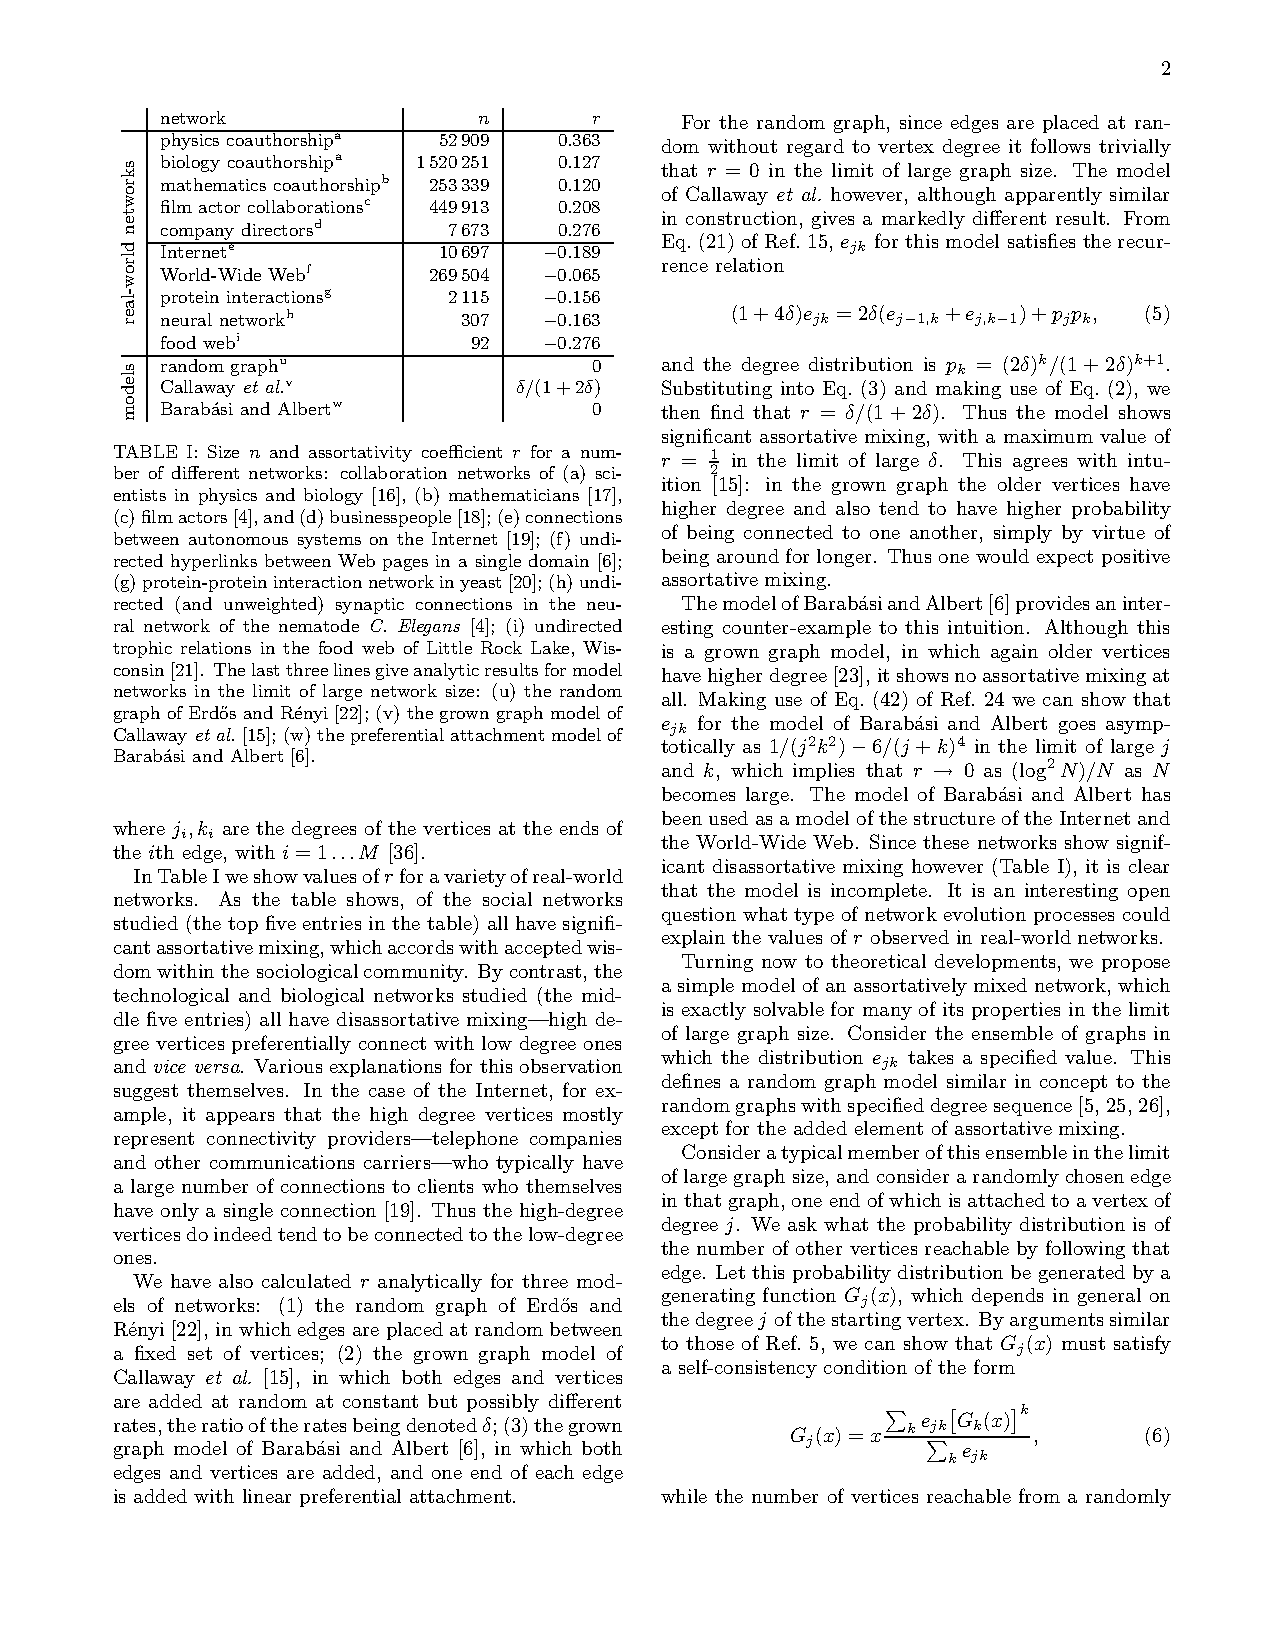
\includegraphics[trim= 1cm 16cm 11cm 1cm, clip=true, width=.5\linewidth]{assortative_mix.pdf}
\end{figure}
{\footnotesize Fuente: \cite{newman2002assortative}}
\end{frame}

\section{Centralidad}

\begin{frame}
\frametitle{Centralidad}
\framesubtitle{Comparaci\'on de tipos de centralidad}
\begin{figure}
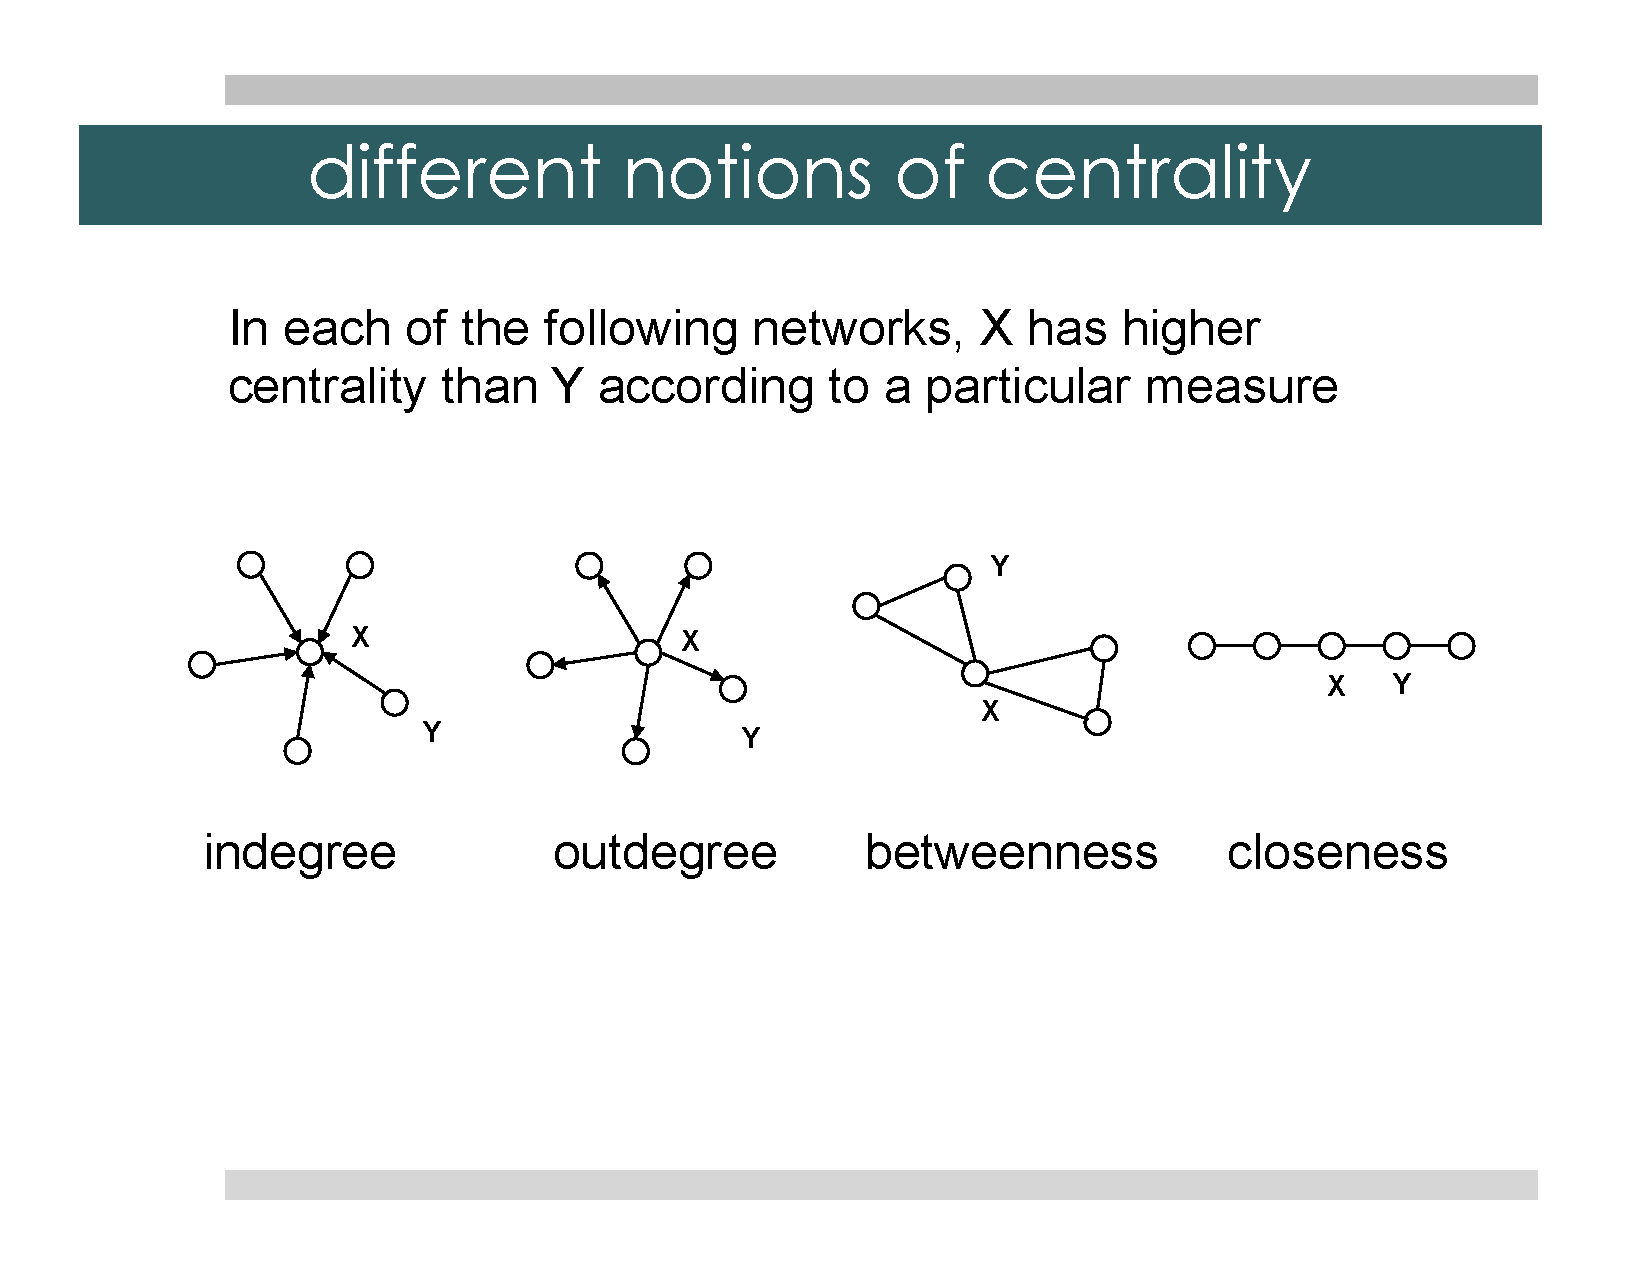
\includegraphics[trim=2cm 6cm 2cm 4cm, clip=true, width=\linewidth]{Lecture3Acentrality_comparison.pdf}
\end{figure}
{\footnotesize Fuente: Extraido de \emph{The structure and function of complex networks}, Newman (2003) \cite{newman2003structure}}
\end{frame}

\begin{frame}
\frametitle{Centralidad}
\framesubtitle{Intermediaci\'on (betweeness)}

\begin{quote}
[betweenness centrality] Se define como la porci\'on de veces que el nodo $i$ necesita al nojo $k$ (sobre
el cual se est\'a midiendo la centralidad) para alcanzar al nodo $j$.
Espec\'ificamente, si $g_{ij}$ es el n\'umero de rutas de $i$ a $j$, y $g_{ikj}$
es el n\'umero de geod\'esicas que pasa por el nodo $k$, entonces la centralidad
de intermediaci\'on est\'a dada por: 
\end{quote}

\begin{equation}
C_B=\sum_i\sum_j{\frac{g_{ikj}}{g_{ij}}}, i \neq j \neq k
\end{equation}

\begin{quote}
En t\'erminos sencillos, [...] b\'asicamente cuenta el n\'umero de geod\'esicas
que pasan a trav\'es del nodo $k$. \cite{borgatti2005centrality}
\end{quote}
\end{frame}

\begin{frame}
\frametitle{Centralidad}
\framesubtitle{PageRank}
\begin{figure}
\centering
\includegraphics[width=.8\linewidth]{PageRank-hi-res}
\end{figure}
{\footnotesize Caricatura de PageRank}
\end{frame}

\section{Importar datos a Gephi}

\begin{frame}
\frametitle{Importad datos a Gephi}
Existen varias formas de importar datos a Gephi:
\begin{itemize}
\item {\bf GEXF} Formato XML, soporta atributos din\'amicos y est\'aticos + jerarqu\'ia \url{http://gexf.net}.
\item {\bf GDF} Texto plano \url{http://guess.wikispot.org/The_GUESS_.gdf_format}.
\item {\bf Pajek NET} Formato de pajek, texto plano \url{http://netwiki.amath.unc.edu/DataFormats/PajekNetAndPajFormats}
\item {\bf UCINET} \url{http://www.analytictech.com/networks/dataentry.htm}
\item {\bf Archivos CSV} los revisaremos en breve...
\end{itemize}
\end{frame}

\begin{frame}
\frametitle{Importar datos a Gephi}
\framesubtitle{Pasos a seguir}

Una manera de importar datos a Gephi es a trav\'es de archivos delimitados por
comas (CSV). Para hacerlo son necesarios dos archivos, uno con v\'ertices y otro
con arcos.

Pasos seg\'un \cite{cherven2013network}

\begin{enumerate}
\item Crear un archivo de {\bf v\'ertices} cuyo contenido es:
  \begin{enumerate}
  \item Identificador.
  \item N\'umero de identificaci\'on
  \item Etiqueta
  \end{enumerate}
\item Crear un archivo de {\bf arcos} cuyo contenido es:
  \begin{enumerate}
  \item Origen
  \item Destino
  \item Tipo (directed/undirected)
  \item N\'umero de identificaci\'on
  \item Etiqueta
  \end{enumerate}
\item Guardar ambos archivos en formato .csv
\item Abrir Gephi y dirigirse al \emph{laboratorio de datos}, lugo clickear en
\emph{Importar archivo de nodos} y \emph{Importar archivo de arcos}.
\end{enumerate}
\end{frame}

\section{Referencias}
\begin{frame}[allowframebreaks]
\footnotesize
\frametitle{Referencias}
\bibliographystyle{plain}
\bibliography{../bib}
\end{frame}


\end{document}

